% Generated by thesis/ch7/exp2/make_assets.py -- do not edit by hand.
\begin{figure}[tbp]
  \centering
  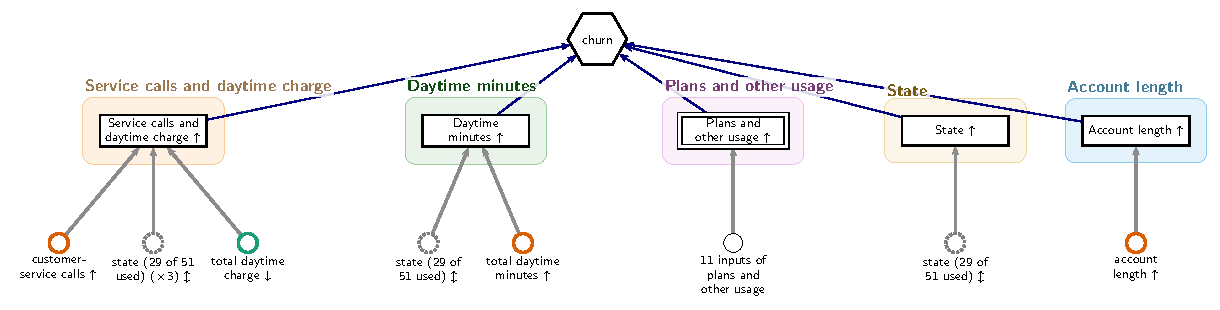
\includegraphics[width=\textwidth]{figures/exp2/exp2-worked-net-concept}
  \caption{Churn seed 5 at the level of concepts: the explanation's 5 top-level parts, each collapsed into one box (\emph{Service calls and daytime charge}; \emph{Daytime minutes}; \emph{Plans and other usage}; \emph{State}; \emph{Account length}), the inputs each reads, and their sum, the churn score, at the top. Arrows on inputs and boxes: the direction of the effect on the final prediction (up raises it, down lowers it, double arrow depends). Edges: blue, a positive weight (raises the score); red, a negative weight; thicker, a larger weight; grey, the inputs a collapsed part reads (no single weight). A grouped input (state) stands for its used levels.}
  \label{fig:exp2-worked-net-concept}
\end{figure}
